In this section, we introduce the proposed approach~\dname~ which learns causal rules for KG link prediction.
\dname~ first transforms the relational data into the propositional data to conduct statistical analysis (Sec. \ref{sec:tabularnizar}).
Then \dname~ presents a local causality identification algorithm based on the $d$-seperation criterion to efficiently mines interpretable causal rules (Sec. \ref{sec:discovery}).
Finally, a specific causation-based score is applied in predictor to answer the queries with learned causal rules (Sec. \ref{sec:link_pred}).
The pipeline of \dname~is illustrated in Fig. \ref{fig:framwork}.
% the proposed CFLP first transforms the input data from graph representation into tabular representation for better  (Sec. \ref{sec:tabularnizar}). Then we design a local causality identification algorithm based on the $d$-seperation criterion to efficiently mines interpretable causal rules (Sec. \ref{sec:discovery}).
% Finally, a specific link prediction approach is applied to integrates the weight information  derived from the causality test (Sec. \ref{sec:link_pred}).
\begin{figure*}[htbp]
\begin{center}
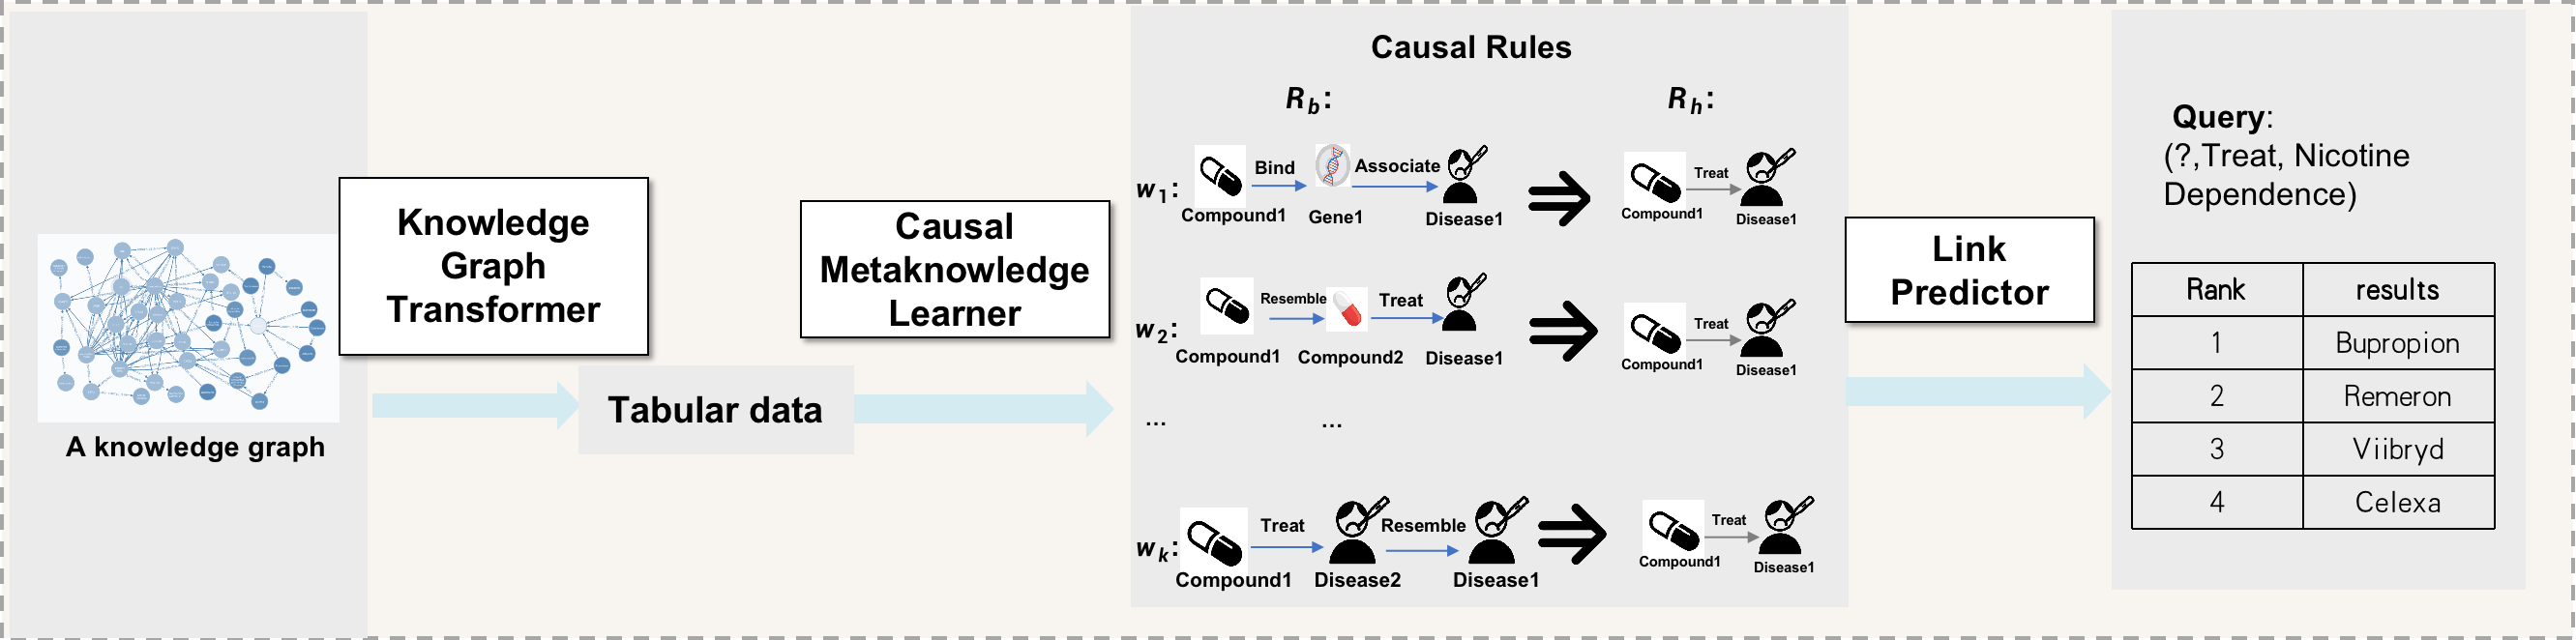
\includegraphics[width=18cm]{submissions/causal-meta-knowledge/figures/cmlp.png}
\end{center}
\caption{The framework of~\dname. Particularly, CFLP first transforms the relational data into propositional data for better statistical analysis. Then it mines interpretable causal rules, which can be interpreted as a kind of metaknowlege\cite{evans2011metaknowledge}.
Finally, a plausibiliy score derived from the causality test is applied in predictor to rank the answers of the given query.}
\label{fig:framwork}
\end{figure*}
\begin{figure*}[hbp]
\begin{center}
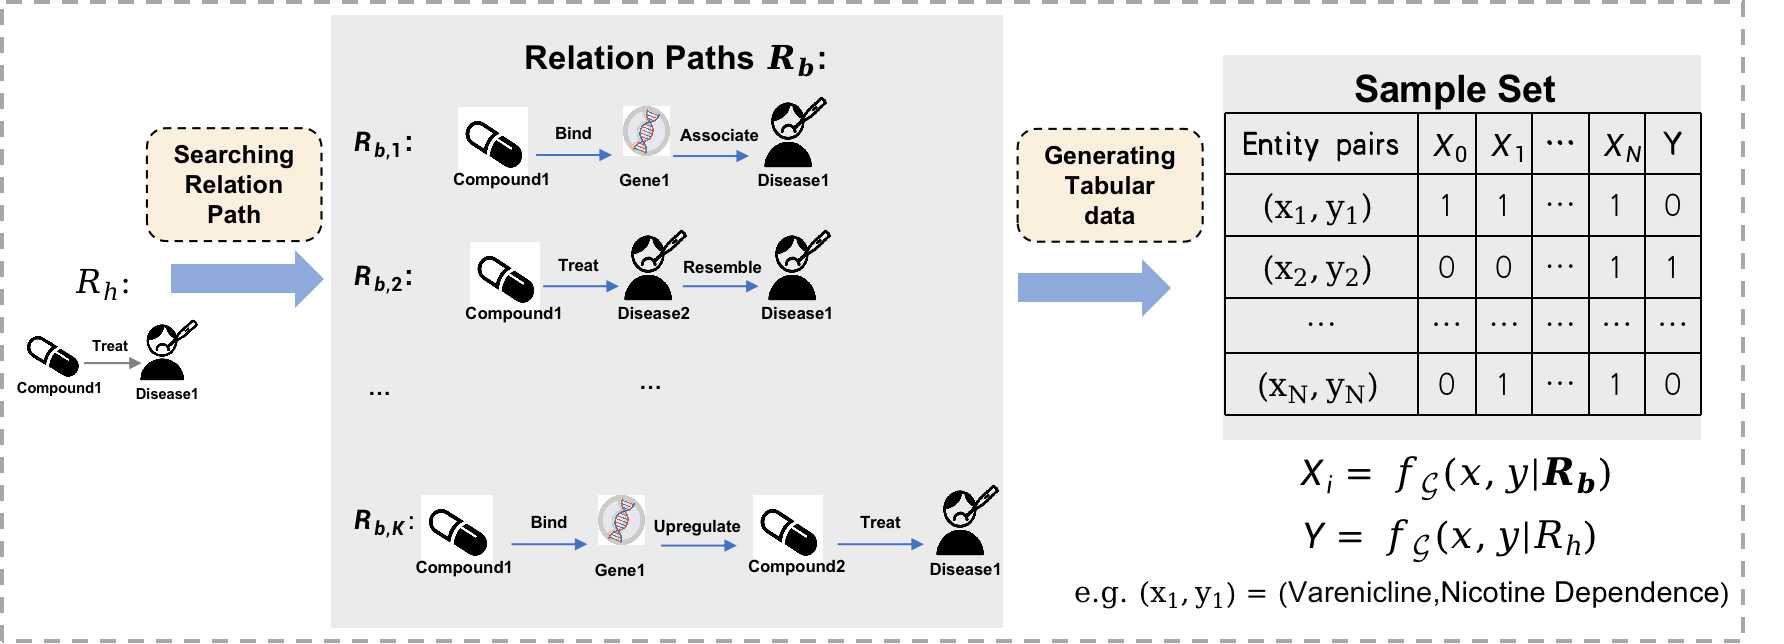
\includegraphics[width=14cm]{submissions/causal-meta-knowledge/figures/transformer.jpg}
\end{center}
\caption{The process of knowledge graph transformer}
\label{fig:tabular}
\vspace{-0.6cm}
\end{figure*}

\subsection{Knowledge Graph Transformer}
\label{sec:tabularnizar}
% The inference rules are generally defined at the concept level, and the link prediction tasks are operated at the entity level.
% For example, based on the inference rule of relation \texttt{Treats(Compound, Disease)}, we can conduct a specific query $(?, Treat, Nicotine Dependence)$.
% In~\dname, to learn the conceptual causal rules, we first introduce the possible causes of a conceptual fact.
Traditional causal discovery algorithms are defined on propositional data, with well-defined variables and samples, which do not exist in relational data like KGs.
Therefore, we give the definition and scope of the variables we study in the causal discovery phase by mapping the potential causes and queried relations into variables.
Then we give the practical approach for transforming KG into tabular data, whose horizontal axis are the variables we defined.
The process is shown schematically in Fig.~\ref{fig:tabular}



\subsubsection{Causal variables in KG}
The causal rule can be interpreted as a description of causal relationship between the body and the head.
Naturally, we formulate variables based on the elements of rules.
% Due to the difficulty of data acquisition, for knowledge graphs extracted from texts, there is often no corresponding attribute information of entities corresponding to them.
% The connection information between a pair of entities is the only source we can access to infer the missing link between them.
% For example, the genetic connection structure is
%$Compound \stackrel{Bind}{\longrightarrow} Gene \stackrel{Associate}{\longrightarrow} Disease$.
% $Bind(Compound, Gene) \circ Associate(Gene, Disease)$.

% \yym{a sample to explain this model}
% \yym{rewrite}
% Relational causal model (RCM) is a Baysian network, which encodes the causal dependency for the relational data.
% RCM is designed for the relational database, in which the entity classes and relations are represented as tables with attributes.
% RCM depends on the known relational skeleton, which includes all the relations between entities, to infer the unknown attributes.
% However, in practice, the relations among entities are missing and are treated as learned target in some application, such as link prediction task for KG.
% And normally, the attributes of entity classes are lack in the real KG.
% Therefore in this section, we will build a causal model for the relations in KG without information of the entities' attributes.
% With the relational skeleton, RCM can represents the conditional independent relationship among the attributes of the entity class.

% We first introduce several concepts and definitions, which are the components of our model.

\noindent
% \begin{definition}
% \textbf{Knowledge Graph Schema(KGS.)}
% A KGS $S=(\mathcal{C}^S, \mathcal{R}^S, \mathcal{V},\mathcal{B} )$ is a directed graph, defined on a KG $\mathcal{G}=(\mathcal{E},\mathcal{R},\mathcal{T})$ with relation set $\mathcal{R}^S \in \mathcal{R}$,
% where each vertice $v \in \mathcal{V}$ corresponds to a concept $C \in \mathcal{C}^S$ and each edge $b \in \mathcal{B}$ corresponds to a relation $R  \in \mathcal{R}^S$.
% \end{definition}

%\begin{definition}
%A \textbf{meta structure} connecting source node $n_h$ and target node $n_t$
%$M=(\mathcal{C}_M, \mathcal{R}_M, \mathcal{V},\mathcal{B}, n_h, n_t)$ is a directed graph, defined on a KG $\mathcal{G}=(\mathcal{E},\mathcal{R},\mathcal{T})$ with concept set $\mathcal{C}$, where $\mathcal{V}$ and $\mathcal{B}$ are node set and edge set, respectively, and each node $v \in \mathcal{V}$ corresponds to a concept $C \in \mathcal{C}_M$ each edge $b \in \mathcal{B}$ corresponds to a relation $R  \in \mathcal{R}_M$.

% with relation set $\mathcal{R}_M \in \mathcal{R}$,
% where each vertice $v \in \mathcal{V}$ corresponds to a concept $C \in \mathcal{C}^S$ and each edge $b \in \mathcal{B}$ corresponds to a relation $R  \in \mathcal{R}^S$.
%\end{definition}
% A relation path is a template and proxy of sub-KG that describes a kind of topological relationship between a pair of concepts.
% Therefore, the bodies of rules can be conceived as topology attributes for all concept pairs.
% And the head of the rule is also a special attribute.
% Here we give the some officially definitions to introduce the assumption on the causes of concept-level links in KG.
%The conceptual triple is a kind of meta structure.
%There is a slightly difference with the past definition of meta structure \cite{huang2016meta}: we do not restrict the meta structure to be a directed acyclic graph (DAG), because the direction of the connection from head entity to tail entity may not be unidirectional or directed under different relational semantics, such as $<Compound,Associate,Disease>$\lsx{?}

%\begin{definition}
%A \textbf{Rule-induced Variable} $X=(C_h,C_t).M$ is defined on two concepts $C_h$ and $C_t$ and a meta structure $M$, where $C_h$ and $C_t$ correspond to $n_s$ and $n_t$ in $M$, respectively.
%\end{definition}

\begin{definitionnew}
For entity pair $(x,y)$, its \textbf{Rule-induced Variable} $X_k=f_{\mathcal{G}}(x,y|\mathbf{R_b}^k)$, where $\mathbf{R_b}^k$ corresponds to the rule body in the $k$-th rule $R_h:\mathbf{R_b}^k (k \in \{1, ..., |\mathcal{B}_h|\})$. The assignment function $f_{\mathcal{G}}(\cdot|\mathbf{R_b})$ can be either connectivity feature or path count for $\mathbf{R_b}$ in KG $\mathcal{G}$.
\end{definitionnew}

The head of rule also induces a special variable $Y=f_{\mathcal{G}}(x,y|R_h)$.
In the real link prediction task, the queries are normally on a specific relation, such as \texttt{Treat} in drug repurposing.
Therefore, the causal rule mining problem is to discovery the causal relationship between variables $X_k=f_{\mathcal{G}}(x,y|\mathbf{R_b}^k), k \in \{1, ..., |\mathcal{B}_h|\}$ and variable  $Y=f_{\mathcal{G}}(x,y|R_h)$.
% With the definition of variables, the causal rule discovery is transformed to the traditional causal discovery task
Then we introduce the practical approach that we transform the KG into tabular data for causality analysis.

% In this paper, we treat the \textit{entity pair} as the study unit, since we focus on the generation mechanism of the relations in KG without the attributes of a single entity and each relation must involve two entities.
% The concept pair label the classes of the entity pair, and the meta structure $M$ reflect the connection characteristics between the two entities. Besides, We assume the concept-level connection information of given concept pair as the factors, which potentially \textit{cause} the specific relation between these two concepts.

%\begin{assumption}
%\textbf{Candidate causes of conceptual triples:}
%\label{ass:candidata}
%given a variable $(C_h,C_t).M_q$ defined by a queried conceptual triple $M_q=<C_h,R,C_t>$, the candidate causes of it are any variables $(C_h^c,C_t^c).M_c$ defined by the meta structure $M_c=(\mathcal{C}_M, \mathcal{R}_M, \mathcal{V},\mathcal{B}, n_h, n_t)$, where $C_h^c=C_h$ and $C_h^t=C_t$.
% and $C_1^{Ca} \cap C_1 \neq \emptyset, C_2^{Ca} \cap C_2 \neq \emptyset$.
%\end{assumption}

% \begin{assumption}
% \textbf{Candidate causes of rule-induced variables:}
% \label{ass:candidata}
% given a variable $X_k=f_{\mathcal{G}}(x,y|\mathbf{R_b}^k)$ defined by the $k$-th rule to reason queried relation $R_th$, the candidate causes of it are any variables $X_j=f_{\mathcal{G}}(x,y|\mathbf{R_b}^j)$ defined by other rule $j(j\neq k)$ in the rule space.
% % and $C_1^{Ca} \cap C_1 \neq \emptyset, C_2^{Ca} \cap C_2 \neq \emptyset$.
% \end{assumption}

% A KGS-based variable $X=f(\mathcal{G},S,e^h,e^t)$ is a function of two entity variables $e^h,e^t$, with each entity variable corresponding to two nodes of KGS $S=(\mathcal{C}^S, \mathcal{R}^S, \mathcal{V},\mathcal{B} )$, where the KGS is defined on KG $\mathcal{G}$.


% \begin{itemize}
%     \item a set of meta structural attributes$(C_h,C_t).\mathcal{M}$
%     \item a set of parents $\text{Pa}((C_h,C_t).M)=\{(U_1,\dots,U_l\}$, where each $U_i$ has the form $C_h,C_t).M_i$;
%     \item a conditional probability distribution (CPD) that represents $P(C_h,C_t).M| C_h,C_t).M)$
% \end{itemize}
% A KGS-based dependency model $\mathcal{M}_\theta$ has two parts:

% 1. The structure $\mathcal{M}=(\mathcal{V},\mathcal{D})$: a directed graph with each node corresponding to a KGS-based variables $X \in \mathcal{V}$ and each edge corresponding to a schema-level dependency defined between two variables in $V$.

% 2. The parameters $\theta$: a conditional probability distribution
% \begin{equation}
% \begin{aligned}
% P(X=f(\mathcal{G},S^X,e^h,e^t)|\text{~parents}(X))
% \end{aligned}
% \end{equation}
% for each KGS-based variable with the entity variables and $\text{parents}(X)=\{Y|Y=f(\mathcal{G},S^Y,e^h,e^t)\}$ is the set of parent KGS-based variables, which have the same entity variable pair with $X$.




% Given the entity set, if we can model the





% \noindent
% \begin{definition}
% \textbf{KGS-based variable}
% A KGS-based variable $X=f(\mathcal{G},S,e^h,e^t)$ is a function of two entity variables $e^h,e^t$, with each entity variable corresponding to two nodes of KGS $S=(\mathcal{C}^S, \mathcal{R}^S, \mathcal{V},\mathcal{B} )$, where the KGS is defined on KG $\mathcal{G}$.
% \end{definition}

% The mapping function $f$ is as following:
% $$
% f(\mathcal{G},S,E^h,E^t)=\left\{
% \begin{aligned}
%     1  & \text{~~if there is an instance path of KGS~}
%        S \text{~with~} e^h,e^t \text{in} \ \mathcal{G}.\\
%     0 & \text{~~otherwise}.
% \end{aligned}
% \right.
% $$


% \begin{definition}
% \textbf{Schema-level dependency}
% A schema-level dependency $Y \to X$, defined between two KGS-based variables $X=f(\mathcal{G},S^X,e^h,e^t)$ and $Y=f(\mathcal{G},S^Y,e^h,e^t)$, is a directed probabilistic dependence from  $Y$ to $X$, which have the same entity variables.
% \end{definition}

% \begin{definition}
% \textbf{KGS-based dependency model}
% A KGS-based dependency model $\mathcal{M}_\theta$ has two parts:

% 1. The structure $\mathcal{M}=(\mathcal{V},\mathcal{D})$: a directed graph with each node corresponding to a KGS-based variables $X \in \mathcal{V}$ and each edge corresponding to a schema-level dependency defined between two variables in $V$.

% 2. The parameters $\theta$: a conditional probability distribution
% \begin{equation}
% \begin{aligned}
% P(X=f(\mathcal{G},S^X,e^h,e^t)|\text{~parents}(X))
% \end{aligned}
% \end{equation}
% for each KGS-based variable with the entity variables and $\text{parents}(X)=\{Y|Y=f(\mathcal{G},S^Y,e^h,e^t)\}$ is the set of parent KGS-based variables, which have the same entity variable pair with $X$.

% \end{definition}


% \noindent
% \begin{definition}
% \textbf{Instances of KGS-based variable}
% A instance of a KGS-based variable $X(S,v^h,v^t)$ is an entity pair $(e^h, e^t)$, with $e^h$ belonging to the concept which $v^h$ corresponds to and $e^t$ belonging to the concept which $v^t$ corresponds to.
% \end{definition}






% In the last section, we introduce the SPRM, which is a Bayesian model defined on the meta structural variables.
% In this section, we will presents the practical method to learn the SPRM $\Pi$ from a given KG.
% Especially, we focus on the learning of the structure $\mathcal{S}$.
% Because structure $\mathcal{S}$ is the fundamental of parameter $\mathcal{S}$ in SPRM, and the exploration of model parameters demands assumptions on the probability distribution followed by the data, hence limiting the applicability of the model.
% In the next section, we will show the structural information is already available for downstream tasks such as link prediction.
% The architecture of the structure learning method is shown in Fig~\ref{fig:framwork}.


% \subsection{Knowledge Graph Tabularnizar}

% \begin{wrapfigure}{r}{0.2\texotwidth}
% \includegraphics[width=0.2\textwidth]{./fig/path_examplev2.pdf}
% \caption{An illustrative KGS, which includes four concepts and three relations.}
% \label{fig:path_example}
% \end{wrapfigure}


% The traditional causal discovery algorithm aims to learn the whole causal structure, without any prior knowledge about the skeleton of the structure or the orientation of the causal relationship.
% which includes all causal relationships between the involved variable.
% The causal structure can be represented as a DAG, where each node indicates an involved variable.
% Discovering causal relationships from observational data
% by a set of causal relationships among a set of variables, and the causal discovery is normally regarded as a the problem of learning the \textit{whole} causal structure from observational data in the prior works.
% However, the fundamental tasks in KG, such as KG completion and KG reasoning, mainly concern the single relation.
% Therefore, the main goal of rule mining is to find the body structure for a given head relation.
% Consequently, in this paper, we only need to solve a \textit{local} causal discovery problem, which is to find all the direct causes for a given KGS-based variable.
% Here we propose an efficient causal rule discovery method, \textit{\dname}, which performs the following steps:
\subsubsection{Transforming knowledge graph into propositional data}

% \begin{figure}[t]
% \centering
% \includegraphics[width=0.45\linewidth]{./figures/path_examplev2.pdf}
% \caption{An illustrative meta structure, which includes four concepts and three relations.}
% \label{fig:path_example}
% \end{figure}

(1) Step-1: Searching candidate causes $X$.
According to definition~\ref{def:horn_rule}, any rule-induced variable $X$, which is defined on entity pair$(x,y)$ and seeks to help reasoning over $R_h$, is a valid candidate cause for $Y=f_{\mathcal{G}}(x,y|R_h)$.
% Further we observed the following phenomena:
% \begin{itemize}
% \item[1)] Any graph contains two specific nodes can be represented as a path between them (duplicate nodes are permitted).
% For example, as shown in Fig.\ref{fig:path_example}, the structure between $C_1$ and $C_2$ can be determined by the path $C_1 \stackrel{R_1}{\longrightarrow} C_2 \stackrel{R_3}{\longrightarrow} C_4 \stackrel{R_3}{\longleftarrow} C_2 \stackrel{R_2}{\longrightarrow} C_3$.
% \item[2)] A complex meta structure can be considered as a combination of multiple meta paths.
% For example, the meta structure $M_N$ in Fig.~\ref{fig:tabular} can be decomposed into two meta path(shown in Fig.~\ref{fig:decompose}).
% The causal function $(C_h,C_t).M_q=f((C_h,C_t).M_N)$ can be represented by
% $(C_h,C_t).M_q=f((C_h,C_t).M_{N_1},(C_h,C_t).M_{N_2})$
% \begin{figure}[t]
% \centering
% 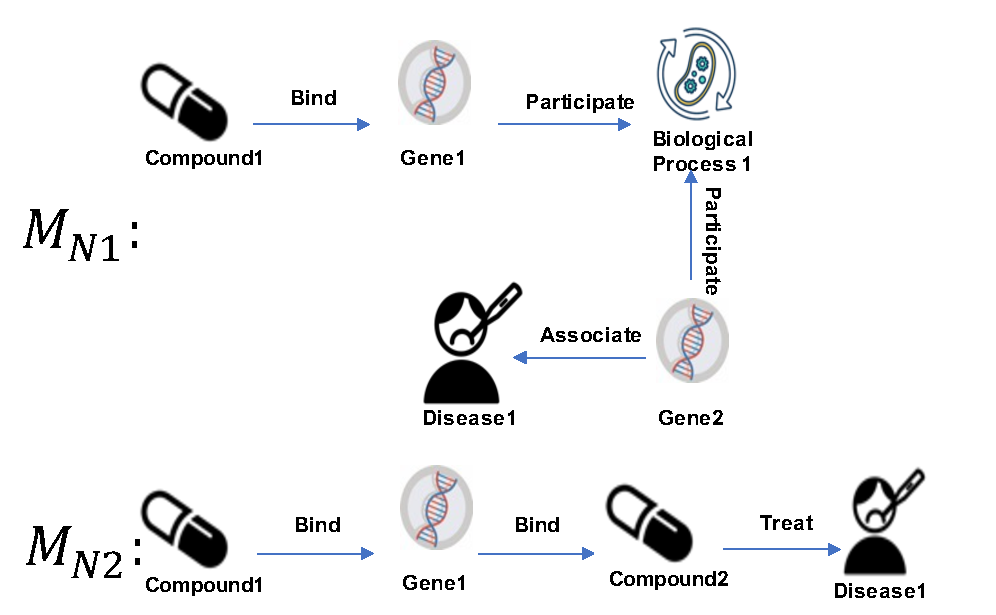
\includegraphics[width=0.8\linewidth]{./figures/decompose.pdf}
% \caption{Two meta paths decomposed from the meta structure $M_N$ in Fig.~\ref{fig:tabular}.}
% \label{fig:decompose}
% \end{figure}
% \begin{equation}
% \label{eq:decompose_meta_path}
% \begin{aligned}
% M_{N_1}:Compound1 \stackrel{Bind}{\longrightarrow}Gene1\stackrel{Participate}{\longrightarrow} Biological Process1 \stackrel{Participate}{\longleftarrow} Gene2\stackrel{Associate}{\longrightarrow} Disease1 \\
% M_{N_2}:Compound1 \stackrel{Bind}{\longrightarrow}Gene1\stackrel{Upregulate}{\longrightarrow} Compound1 \stackrel{Treat}{\longleftarrow}Disease1.
% \end{aligned}
% \end{equation}
% $M_{N_1}:Compound1 \stackrel{Bind}{\longrightarrow}Gene1\stackrel{Participate}{\longrightarrow} Biological Process1 \stackrel{Participate}{\longleftarrow} Gene2\stackrel{Associate}{\longrightarrow} Disease1$ and $M_{N_2}:Compound1 \stackrel{Bind}{\longrightarrow}Gene1\stackrel{Upregulate}{\longrightarrow} Compound1 \stackrel{Treat}{\longleftarrow}Disease1$.
% \item[2)]  There are many well-studied path finding algorithms, which can search the paths under different types of constraints, such as Dijkstra’s algorithm~\cite{lanning2014dijkstra}, A* search~\cite{cui2011based}, best-first search~\cite{heusner2018best}, etc.
% These off-the-shelf methods can be directly adopted to our framework.
% In the experiments, we adopt the best-first search algorithm.
% \item[3)] Lots of existing rule mining methods~\cite{sadeghian2019drum,yang2017differentiable,ho2018rule} designed for the \textit{closed rules}, meaning that each entity set appears in at least two edges of the rule.
% It renders the path-like graph structure in most cases.
% \end{itemize}
So we find all the candidate causes by searching all the paths between entity pairs $(x, y)$, which have the relation $R_h$ between them.
There are many well-studied path finding algorithms, which can search the paths under different types of constraints, such as Dijkstra’s algorithm~\cite{lanning2014dijkstra}, A* search~\cite{cui2011based}, best-first search~\cite{heusner2018best}, etc.
% These off-the-shelf methods can be directly adopted to our framework.
In the experiments, we adopt the best-first search algorithm.
Since the number of candidate causes can be the power level of the number of relation types, we require that the length of the path is no more than $\ell$, where $\ell$ is the hyper-parameters.
In the experiments of this paper, we set $\ell$ as 3.
% need to be supported by at least $a_{sup}$ entity pair $(e^h,e^t)$ in the training KG, and the length of the path is no more than $\ell$, where $a_{sup}$ and $\ell$ are the hyper-parameters.
(2) Step-2: generating samples.
% In tabular data, variables have distinct physical meanings, and the values of each instance are accessed via data collection.
% There is no explicit quantitative information inside triple-based knowledge graphs.
% For further causality learning, the assignment rules for the variables specified by structural attributes must be agreed upon in order to generate a numerical sample set that can be statistically analyzed.
In this paper, we use the connectivity as the assignment function to get quantitative samples.
\noindent
\begin{definitionnew} the
\textbf{binary assignment function of rule-induced variable} is as following:
$$
f_\mathcal{G}(e_h,e_t|\mathbf{R_b}^k)=\mathbbm 1_{\rm con}(e_h,e_t|\mathbf{R_b}^k)
$$
where $\mathbbm 1_{\rm con}(e_h,e_t|\mathbf{R_b}^k) \in \{0,1\}$ checks whether there exists a path instance of $\mathbf{R_b^k}$ between $e_h$ and $e_t$ in KG $\mathcal{G}$.
\end{definitionnew}

% \begin{definition} the
% \textbf{binary assignment function of meta structural attribute-defined variable} is as following:
% $$
% f_{\mathcal{G},(C_h,C_t).M}(e_h,e_t)=\left\{
% \begin{aligned}
%     1  & \text{~~if condition one is satisfied}. \\
%     0 & \text{~~otherwise}.
% \end{aligned}
% \text{for~} e_h \in
%     \mathcal{E}_h \text{~and~} e_t \in \mathcal{E}_t\\
% \right.
% $$
% where condition one is there is an meta structure instance of $M$ between $e_h$ and $e_t$ in KG $\mathcal{G}$.
% \end{definition}

In this assignment function, we consider whether two entities can be connected via a relation path, instead of the entities or number of the connection paths.
There are two main reasons for this design:
(1) We expect that the mined causal relationship can be generalized to any dataset in this domain.
% Without the attribute of the entities, we can not model the entities based on the their common features.
Thus, if we want to distinguish different entities which instantiate the meta structure, we need to build a multinomial model for all possible entities.
The multinomial would be infeasibly large.
And our model can not be applied to any scenario which contain an unseen entity.
(2) this function can be seen as an aggregation function to summary the connection information between entities.
The aggregation function is very common in the causal relation model~\cite{maier2010learning,lee2016learning,lee2020towards,salimi2020causal}.
With the aggregation function, we can build a concise and expressive model.
Since the only thing we need is whether the entities are connected.
Based on this assignment function, by sampling entity pairs in the training KG and querying the corresponding variable values, we can obtain tabular data for causal analysis.




% (2) Step-2: Refinement of the Identical Relations.
% In KG, there may be some identical relations, even though they have different relation names.
% For example, Wife(A,B) $\leftrightarrow$ Husband(B,A), if A is the wife of B, then B must be the husband of A.
% However, they will lead the invalid independence test in the following causal discovery step, even though these two relations have very strong causal relationship with each other.
% In particular, based on the causal variable and sample definitions in KG (Sec.~\ref{sec:v_a_s}), these two relations are the same variables for the causal discovery method, since the values of their samples are the same all the time.
% When one relation is treated as the conditional variable in the independent test of the other one, the conditional independence (CI) test $CI(X,Y|X)$ will be judged as independent.
% So for an analyzed KGS $S_E$, we search all the identical KGSs in the input KG and temporarily remove them from the candidate cause set in the independent test period.
% The causal rules which include the identical KGSs will have the highest weight, when they are applied into the downstream tasks.
\subsection{Causal MetaKnowlege Discovery via $d$-seperation Criterion}
\label{sec:discovery}

The $d$-separation criteria~\cite{glymour2016causal} (see Definition 3.4) is a sufficient and necessary condition for the compatibility of a probability distribution with a causal model in the form of a directed acyclic graph (DAG).
It states that a joint probability distribution of a set of random variables is compatible with the DAG (each node represents one of the given variables and each arrow represents the possibility of causal influence) if and only if the distribution satisfies a set of conditional independence relations encoded in the structure of the DAG.
Therefore, $d$-separation is widely used in the algorithms in discovering causal structure\cite{giudice2022dual,sondhi2019reduced,gerhardus2020high}.

\begin{definitionnew}
\textbf{d-seperation.} A path $p$ is blocked by a set of nodes $Z$ if and only if:

1.$p$ contains a chain of nodes $A \to B\to C$ or a fork $A \gets B\to C$ such that the middle node $B$ is in $Z$ (i.e., $B$ is conditioned on), or:

2. $p$ contains a collider $A \to B \gets C$ such that the collision node $B$ is not in $Z$, and no descendant of $B$ is in $Z$.

If $~Z$ blocks every path between two nodes $X$ and $Y$, then $X$ and $Y$ are $d$-separated, conditional on $Z$, and thus are independent conditional on $Z$.
\end{definitionnew}


\begin{algorithm2e}
\caption{Local causal metaknowledge discovery}
\label{alg:pc-like}
\KwIn{$Y$ and $\{y_i\}, i=1,\dots,N$ : variable and samples of queried variable $(C_h,C_t).M_q$ ;
 $\mathcal{X}^{Ca} = \{X_k\}, k=1,\dots,K$ and $\{\{x_i\}_k\}, i=1,\dots,N$: variables and samples of candidate causes; }
\KwOut{causes $\mathcal{X}^{C}$ of $Y$}
level $d \gets 0$\;
\While{$d<= |\mathcal{X}^{Ca}|-1$}{

\For{each $X_k \in  \mathcal{X}^{Ca}$}{
    \For{each subset $\mathcal{Z} \in \mathcal{X}^{Ca} \backslash \{ X_k\}$ and $|\mathcal{Z}|=d$}{
    Test CI($X_k,Y|\mathcal{Z}$)\;
    \If{CI($X_k,Y|\mathcal{Z}$)}{
        Test CI($\mathcal{Z},Y|X_k$) {(Reverse CI test.)} \;
        \If{not CI($\mathcal{Z},Y|X_k$)}{
            Remove $X_k$ from $\mathcal{X}^{Ca}$\;
            Break\;
        }
    }
}
}
$d \gets d+1$\;
}
$\mathcal{X}^{C} = \mathcal{X}^{Ca}$
\end{algorithm2e}

In this work, we design an efficient causal metaknowledge discovery algorithm based on $d$-separation.
With $d$-separation, we can get the following conclusion: given any set of variables $Z$, where $Z$ does not include $X$, $X$ is not independent of its parent node ({i.e.} direct cause).
% \yym{theorem}
Based on this conclusion, we can obtain a criterion for determining the direct cause of variable $X$.
Furthermore, we design the following local causal metaknowledge discovery algorithm (Algo.~\ref{alg:pc-like}) for the queried variable $Y=f_{\mathcal{G}}(x,y|R_h)$.
We only mine the direct cause of $Y$, instead of the entire causal structure of variable set $\mathcal{X}^{Ca} \cup \{Y\}$.
Particularly, given a queried variable $Y=f_{\mathcal{G}}(x,y|R_h)$, for each candidate cause in $\mathcal{X}^{Ca}$~(denoted as variable $X_k$),
the proposed algorithm decides whether $X_j$ should be retained in candidate causes set $\mathcal{X}^{Ca}$ by testing the independence of $X_k$ and $Y$ conditioning on a subset $\mathcal{Z}$ of $\mathcal{X}^{Ca}\backslash \{X_k\}$.
The conditional independent(CI) tests are organised by levels (based on the size $d$ of the conditioning sets).
At the first level ($d = 0$), all pairs of variables are tested conditioning on the empty set.
Some of the candidate causes would be removed and the algorithm only tests the remaining candidate causes in the next level ($d = 1$).
The size of the conditioning set, $d$, is progressively increased (by one) at each new level until $d$ is greater than $|\mathcal{X}^{Ca}|-1$.
Each corresponding relation path of $X \in \mathcal{X}^C$ construct a valid rule to predict the relation $R_h$ in $Y$.

\begin{figure}[t]
\vspace{0cm}
\centering
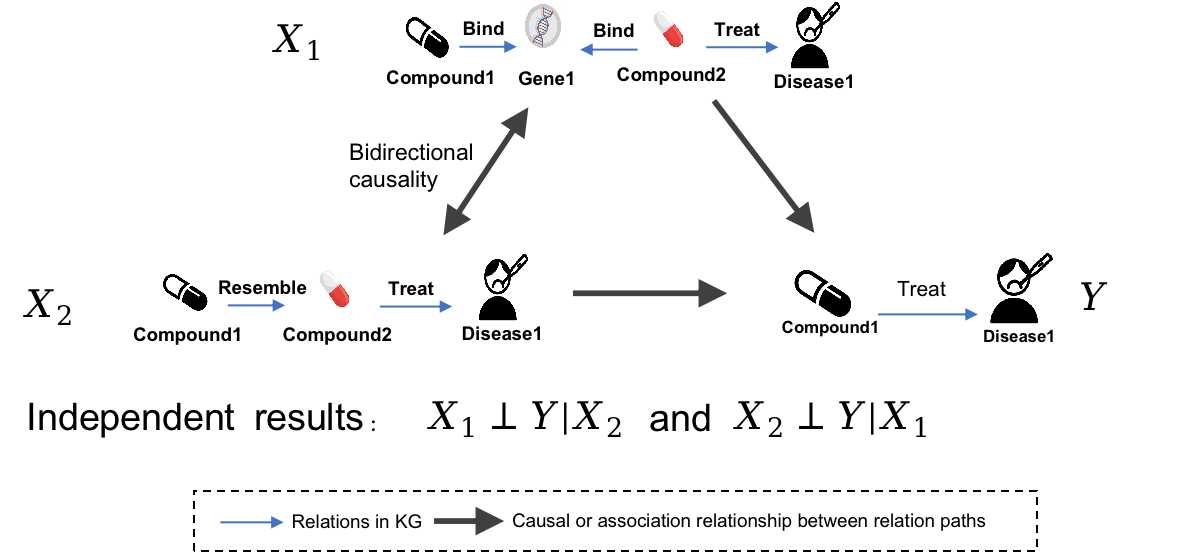
\includegraphics[width=8.5cm]{submissions/causal-meta-knowledge/figures/bidirection.jpg}

\caption{An example of bidirectional causal relationship, which may lead wrong results.}
\label{fig:bidirection}

\end{figure}

It is noteworthy that we add the reverse CI test in Algo.~\ref{alg:pc-like} (line 7) to avoid the impact of redundant relations in KGs.
For example, $Compound1 \stackrel{Resembles}{\longrightarrow}Compound2$ and $Compound1 \stackrel{Binds}{\longrightarrow}Gene1\stackrel{Binds}{\longleftarrow}Compound2$ express the similar message, which could lead the invalid independence test, as shown in Fig.~\ref{fig:bidirection}.
% \xz{As shown in Fig. xx}, the CI test results
% $Y=(C_h,C_t).M_q  \perp  X_1=(C_h,C_t).M_1| X_2=(C_h,C_t).M_2$  and $Y\perp  X_2|X_1$, where $C_h$ is Compound1, $C_t$ is Disease1, $M_q=Compound1 \stackrel{Treats}{\longrightarrow}Disease1$, $M_1= Compound1 \stackrel{Resembles}{\longrightarrow}Compound2 \stackrel{Treats}{\longrightarrow}Disease1$ and  $M_2= Compound1 \stackrel{Binds}{\longrightarrow}Gene1\stackrel{Binds}{\longleftarrow}Compound2 \stackrel{Treats}{\longrightarrow}Disease1$.
It will lead both $X_1$ and $X_2$ are removed from the candidate cause set of queried variable $Y$, even though they have very strong causal relationship with the drug treatment of diseases.
Consequently, we use the reverse CI test to avoid this issue.
In particular, if $X_j$ and $Y$ are judged to be independent conditioning on $\mathcal{Z}$, we will examine the independence between $\mathcal{Z}$ and $Y$ conditioning on $\mathcal{X}_j$.
When the result of the additional test is negative, $X_j$ will be removed from $\mathcal{X}^{Ca}$.
In this paper, we adopt SCI method~\cite{marx2019testing} as the independent test method in the experiments, which works well on limited samples and discrete variables.

\subsection{Link Prediction based on Explainable Causal Metaknowledge}
\label{sec:link_pred}

The approach for link prediction based on interpretable rules tends to generate corresponding weights in the rule mining phase. By accumulating the weights of the rules satisfied by each predicted entity, a score of the predicted entities can be generated, and then the results are ranked based on this score.
Here we first introduce how to generate rule weights under the causal model and then describe the approach for link prediction based on generated weights.

\begin{figure}[t]
\vspace{0cm}
\centering
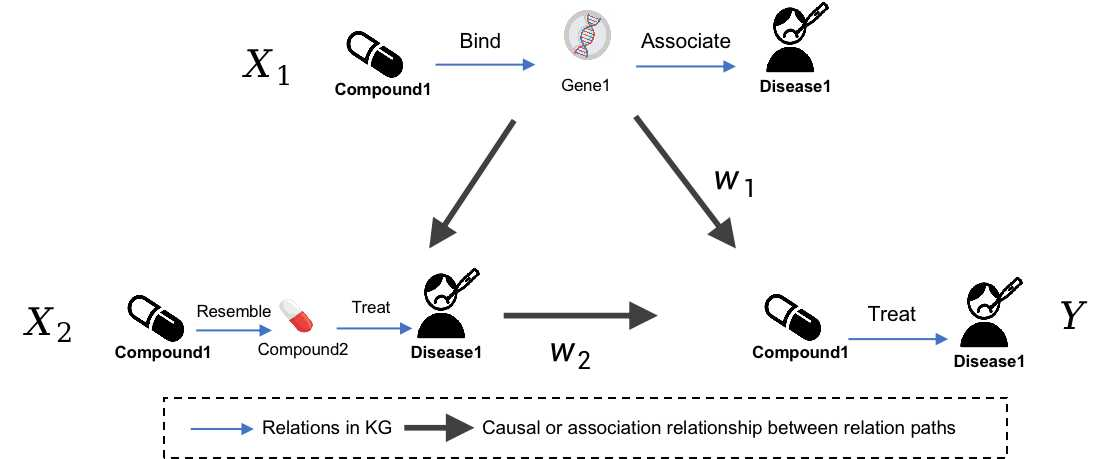
\includegraphics[width=8.5cm]{submissions/causal-meta-knowledge/figures/direct_cause.jpg}
% \vspace{-3pt}
\caption{An example of non-independent rule-induced variables, which are both the causes of queried relation.}
\label{fig:direct_cause_example}
% \vspace{-5pt}
\end{figure}

\noindent
\textbf{Weights of rules based on conditional dependency.}
In Algo.~\ref{alg:pc-like}, we discover the direct causes by the non-independence relationship between the candidate meta structures and the queried meta structures.
It is important to note that the meta structures of $\mathcal{X}^C$ are not independent to each other.
Fig.~\ref{fig:direct_cause_example} gives an example for this case. Specifically, $X_1$ and $X_2$ are both causes of $Y$.
Since $X_1$ is also a cause of $X_2$, if we directly calculate the causal strength between $X_2$ and $Y$, it is inevitable that $w_2$ will contain the causal effects that arise from $X_1$ along the path $X_1\to X_2 \to Y$.
Therefore, in order to better measure the importance of each causal rule and to avoid double-counted in the calculation of each proposed entity's score, we adopt the minimal conditional dependence as a measure of the importance of causal rules:

\begin{equation}
\label{eq:weight}
\begin{aligned}
w_j  = \min(\{ dependence(X_j,Y|\mathcal{Z}) \})
\\
\text{~for any subset~} \mathcal{Z} \in \mathcal{X}^{Ca}\backslash \{X_j\},
\end{aligned}
\end{equation}
where $w_j$  is the rule weight of the meta structure in $X_j$.
In this paper, we use the $SCI_f(X,Y|Z)$ in SCI independence test~\cite{marx2019testing} as the dependence score in Eq.~\ref{eq:weight}, which can be get in the process of causal rules discovery.
The higher of $SCI_f(X,Y|Z)$, the stronger the dependency.

\noindent
\textbf{Score function of entity results.}
Because of the incompleteness nature of KGs, open world assumption (OWA)~\cite{ji2021survey} is often considered on real datasets.
Under the OWA, the SUM function are usually adopted to calculate the ranking score of the predicted entity $e_h$ in link prediction task $(?,R_h,e_t)$:
\begin{equation}
\label{eq:link-prediction-sum}
\begin{aligned}
S_{R_q}^{sum}=\sum_{i=1}^K \tilde{w}_i Q_{i},.
\end{aligned}
\end{equation}
where $K$ is the number of causal rules, $\tilde{w}_i$ is the normalized weight.
$Q_i=1$ when the body of the $i$-th causal rule holds for the entity pair ($e_h, e_t$), otherwise $Q_i=0$.
This approach focuses on the entities supported by multiple rules and does not use the non-existent relations between entity pairs, since the unreliable negative samples under OWA.
In this paper, Eq.~\ref{eq:link-prediction-sum} is used in the link predictions on real data.
For KG under closed world assumption(CWA)~\cite{ji2021survey}, the negative facts are also reliable, therefore we design a new function to apply the rules in the link prediction task.
Particularly, given an query $(?,R_h,e_t)$, the score of the triple $(e_h,R_h,e_t)$ is true can be formulated as:
\begin{equation}
\label{eq:link-prediction-avg}
\begin{aligned}
S_{R_q}^{avg} = \sum_i^K \tilde{w}_i \big(Q_i \bar{Y}_{X_i=1} + (1-Q_i) \bar{Y}_{X_i=0}\big),
\end{aligned}
\end{equation}
where $K$ is the number of causal rules for the queried relation, $\tilde{w}_i$ is the normalized weight for the $i$-th result rule.
$\bar{Y}_{X_i=1}$ denotes the proportion of the queried relation to be true when the body of the $i$-th causal rule is true in the training data, and $\bar{Y}_{X_i=0}$ denotes the proportion of the queried relation to be true when the body of the $i$-th causal rule is false.
$Q_i=1$ when the body of the $i$-th causal rule holds for the entity pair ($e_h$, $e_t$), otherwise $Q_i=0$.
The results will be ranked by $S_{R_q}$ of each valid $e_t$.
In this paper, Eq.~\ref{eq:link-prediction-avg} is used in the link predictions on simulation data.


% For the link prediction $<?,R,e_t>$, there are two ways to calculate the ranking score of the predicted entity $e_h$:
% \begin{itemize}
% %     \item MAX: this approach highlights the role of the highest-impact rule.
% % \begin{equation}
% % \label{eq:link-prediction-max}
% % \begin{aligned}
% % S_{R_q}^{max}=\max \left\{\tilde{w}_{1} Q_{1}, \tilde{w}_{2} Q_{2}, \ldots, \tilde{w}_{K} Q_{K}\right\}.
% % \end{aligned}

%  \item SUM: this approach focuses on the results supported by multiple rules.
% \begin{equation}
% \label{eq:link-prediction-sum}
% \begin{aligned}
% S_{R_q}^{sum}=\sum_{i=1}^K \tilde{w}_i Q_{i},.
% \end{aligned}
% \end{equation}
% where $K$ is the number of causal rules, $\tilde{w}_i$ is the normalized weight.
% $Q_i=1$ when the body of the $i$-th causal rule holds for the entity pair ($e_h, e_t$), otherwise $Q_i=0$.
% \item AVG: \xz{for a $e_t$, this approach considers both the prediction of a rule on the target relation when it is satisfied and unsatisfied.}

% \begin{equation}
% \label{eq:link-prediction-avg}
% \begin{aligned}
% S_{R_q}^{avg} = \sum_i^K \tilde{w}_i \big(Q_i \bar{Y}_{X_i=1} + (1-Q_i) \bar{Y}_{X_i=0}\big),
% \end{aligned}
% \end{equation}
% where $\bar{Y}_{X_i=1}$ denotes the proportion of the queried relation to be true when the body of the $i$-th causal rule is true in the training data, and $\bar{Y}_{X_i=0}$ denotes the proportion of the queried relation to be true when the body of the $i$-th causal rule is false.
% \end{itemize}
% These ranking functions show their unique advantages under different application scenarios, and we provide thorough discussions for them based on the experimental results. 